% small.tex
\documentclass{beamer}
%\usetheme{default}
\usetheme{Warsaw}

\usepackage{tikzsymbols}
\usepackage{tkz-berge, tkz-graph}
\usepackage{caption}
\usepackage{colortbl}

% Define some colors:

%\definecolor{DarkFern}{HTML}{407428}
%\definecolor{DarkCharcoal}{HTML}{4D4944}
%\colorlet{Fern}{DarkFern!85!white}
%\colorlet{Charcoal}{DarkCharcoal!85!white}
%\colorlet{LightCharcoal}{Charcoal!50!white}
%\colorlet{AlertColor}{orange!80!black}
%\colorlet{DarkRed}{red!70!black}
%\colorlet{DarkBlue}{blue!70!black}
%\colorlet{DarkGreen}{green!70!black}


% Use the colors:

%\setbeamercolor{title}{fg=Fern}
%\setbeamercolor{frametitle}{fg=Fern}
%\setbeamercolor{normal text}{fg=Charcoal}
%\setbeamercolor{block title}{fg=black,bg=Fern!25!white}
%\setbeamercolor{block body}{fg=black,bg=Fern!25!white}
%\setbeamercolor{alerted text}{fg=AlertColor}
%\setbeamercolor{itemize item}{fg=Charcoal}


\newcommand{\N}{\mathbb{N}}
\newcommand{\Z}{\mathbb{Z}}
\newcommand{\R}{\mathbb{R}}
\newcommand{\Q}{\mathbb{Q}}

\newcommand{\F}{\mathbb{F}}

\newcommand{\bd}{\textbf}
\newcommand{\on}{yellow}
\newcommand{\off}{white}
\usepackage{mathtools}
\DeclarePairedDelimiter\abs{\lvert}{\rvert}%
\DeclarePairedDelimiter\norm{\lVert}{\rVert}%
\setlength{\jot}{10pt}

\begin{document}


\title[The Cyclic Lightbulb Game] % (optional, only for long titles)
{The Cyclic Lightbulb Game}
%\subtitle{Subtitle}
\author[Hickey, Maier, Wollenweber] % (optional, for multiple authors)
{Claire Hickey, Justin Maier, Josh Wollenweber}
\institute[University of Pittsburgh] % (optional)
{
  \inst{}%
  University of Pittsburgh
}
\date[January 31, 2019] % (optional)
{Math 1800,

January 31, 2019}
\subject{Lightbulb Game}

\frame{\titlepage}

%%%%%%%%%%%%%%%%%%%%%%%%%%%%%%%%%%%%

\begin{frame}
\frametitle{The Lightbulb Game}

We want to turn off the lightbulbs:

\begin{figure}[!h]
    \centering
    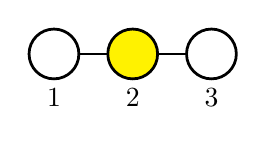
\begin{tikzpicture}
        %\GraphInit[vstyle=Classic]
        \SetVertexMath
        %\tikzset{VertexStyle/.style = {shape = circle,fill = black, minimum size = 5pt,inner sep=0pt}}
        %\SetVertexNoLabel
        \SetVertexLabelOut
        \SetVertexNormal[Shape=circle, FillColor=\off, LineWidth=1pt]
        \Vertex[Lpos=-90]{1}
        \SetVertexNormal[Shape=circle, FillColor=\on, LineWidth=1pt]
        \EA[Lpos=-90](1) {2}
        \SetVertexNormal[Shape=circle, FillColor=\off, LineWidth=1pt]
        \EA[Lpos=-90](2) {3}
        \Edges(1,2,3)
    \end{tikzpicture}
    %\captionsetup{labelformat=empty}
\end{figure}

Pressing a bulb's switch changes the state of the bulb itself and the bulbs directly
adjacent to it. For example, after pressing 1:

\begin{figure}[!h]
    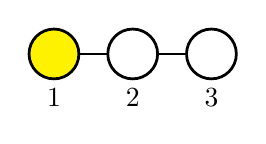
\begin{tikzpicture}
        %\GraphInit[vstyle=Classic]
        \SetVertexMath
        %\tikzset{VertexStyle/.style = {shape = circle,fill = black, minimum size = 5pt,inner sep=0pt}}
        %\SetVertexNoLabel
        \SetVertexLabelOut
        \SetVertexNormal[Shape=circle, FillColor=\on, LineWidth=1pt]
        \Vertex[Lpos=-90]{1}
        \SetVertexNormal[Shape=circle, FillColor=\off, LineWidth=1pt]
        \EA[Lpos=-90](1) {2}
        \EA[Lpos=-90](2) {3}
        \Edges(1,2,3)
    \end{tikzpicture}
\end{figure}

\pause
We can extend this game to $n$ lightbulbs:
\begin{figure}[!h]
    \centering
    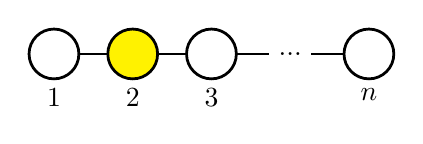
\begin{tikzpicture}
        %\GraphInit[vstyle=Classic]
        \SetVertexMath
        %\tikzset{VertexStyle/.style = {shape = circle,fill = black, minimum size = 5pt,inner sep=0pt}}
        %\SetVertexNoLabel
        \SetVertexLabelOut
        \SetVertexNormal[Shape=circle, FillColor=\off, LineWidth=1pt]
        \Vertex[Lpos=-90]{1}
        \SetVertexNormal[Shape=circle, FillColor=\on, LineWidth=1pt]
        \EA[Lpos=-90](1) {2}
        \SetVertexNormal[Shape=circle, FillColor=\off, LineWidth=1pt]
        \EA[Lpos=-90](2) {3}
        \SetGraphUnit{2}
        \EA[Lpos=-90](3) {n}
        \Edges(1,2,3)
        \Edge[label={...}](3)(n)
    \end{tikzpicture}
    %\captionsetup{labelformat=empty}
\end{figure}
\end{frame}

\begin{frame}
\frametitle{The Lightbulb Game}
\bd{The central question:} When can we always find a solution? 
\end{frame}

\begin{frame}
\frametitle{Converting the Lightbulb Game to a Problem in Linear Algebra}
    We can represent a lightbulb game like the one below with a system of linear
    equations:
    \[
        c_1
        \begin{pmatrix}
            1\\1\\0\\0
        \end{pmatrix}
        + c_2
        \begin{pmatrix}
            1\\1\\1\\0
        \end{pmatrix}
        + c_3
        \begin{pmatrix}
            0\\1\\1\\1
        \end{pmatrix}
        + c_4
        \begin{pmatrix}
            0\\0\\1\\1
        \end{pmatrix}
        =
        \begin{pmatrix}
            0\\0\\1\\1
        \end{pmatrix}
    \]
\begin{figure}[!h]
    \centering
    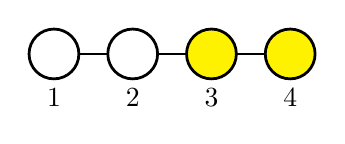
\begin{tikzpicture}
        %\GraphInit[vstyle=Classic]
        \SetVertexMath
        %\tikzset{VertexStyle/.style = {shape = circle,fill = black, minimum size = 5pt,inner sep=0pt}}
        %\SetVertexNoLabel
        \SetVertexLabelOut
        \SetVertexNormal[Shape=circle, FillColor=\off, LineWidth=1pt]
        \Vertex[Lpos=-90]{1}
        \EA[Lpos=-90](1) {2}
        \SetVertexNormal[Shape=circle, FillColor=\on, LineWidth=1pt]
        \EA[Lpos=-90](2) {3}
        \EA[Lpos=-90](3) {4}
        \Edges(1,2,3,4)
    \end{tikzpicture}
    %\captionsetup{labelformat=empty}
\end{figure}
\end{frame}

\begin{frame}
\frametitle{Converting the Lightbulb Game to a Problem in Linear Algebra}

We can represent this in matrix form $Ac=b$, where $b$ is starting configuration, and
the matrix $A$ is
\[
    A=
    \begin{pmatrix}
        1 & 1 & 0 & 0\\
        1 & 1 & 1 & 0\\
        0 & 1 & 1 & 1\\
        0 & 0 & 1 & 1
    \end{pmatrix}
\]
\pause 
To \emph{determine} whether this system always has solution we will use the
\emph{determinant}.
\pause

Recall that the system $Ac=b$ has exactly one solution for every $b$ if and only if
$\abs{A} \neq 0$.
\end{frame}

\begin{frame}
    \frametitle{Calculating the Determinant}

    To calculate the determinant we will make use of cofactor expansion. For example,
    \begin{align*}
        \abs{A} &=
        \begin{vmatrix}
            a_{11} & a_{12} & a_{13}\\
            a_{21} & a_{22} & a_{23}\\
            a_{31} & a_{32} & a_{33}
        \end{vmatrix}\\
        &= a_{11}(-1)^{1+1}
        \begin{vmatrix}
            a_{22} & a_{23} \\
            a_{32} & a_{33}
        \end{vmatrix}
        +
        a_{12}(-1)^{1+2}
        \begin{vmatrix}
            a_{21} & a_{23} \\
            a_{31} & a_{33}
        \end{vmatrix}\\
        &+ a_{13}(-1)^{1+3}
        \begin{vmatrix}
            a_{21} & a_{22} \\
            a_{31} & a_{32}
        \end{vmatrix}
    \end{align*}
\end{frame}

\begin{frame}
    \frametitle{Calculating the Determinant}
    We will also need the determinants of upper and lower triangular matrices:
    \[
        \begin{vmatrix}
            a_{11} & 0 & 0\\
            a_{21} & a_{22} & 0\\
            a_{31} & a_{32} & a_{33}
        \end{vmatrix}
        =
        \begin{vmatrix}
            a_{11} & a_{12} & a_{13}\\
            0 & a_{22} & a_{23}\\
            0 & 0 & a_{33}
        \end{vmatrix}
        = a_{11}a_{22}a_{33}
    \]
    \pause
    This holds for $n$ dimensional triangular matrices as well (can be shown by
    induction).
\end{frame}

\begin{frame}
\frametitle{When is the Linear Lightbulb Game Solvable?}
The matrix for the linear game on $4$ lightbulbs looks like
\[
    \begin{pmatrix}
        1 & 1 & 0 & 0\\
        1 & 1 & 1 & 0\\
        0 & 1 & 1 & 1\\
        0 & 0 & 1 & 1
    \end{pmatrix}
\]

\begin{figure}[!h]
    \centering
    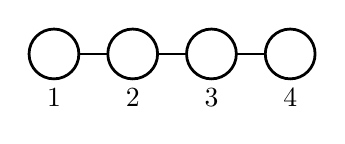
\begin{tikzpicture}
        %\GraphInit[vstyle=Classic]
        \SetVertexMath
        %\tikzset{VertexStyle/.style = {shape = circle,fill = black, minimum size = 5pt,inner sep=0pt}}
        %\SetVertexNoLabel
        \SetVertexLabelOut
        \SetVertexNormal[Shape=circle, FillColor=\off, LineWidth=1pt]
        \Vertex[Lpos=-90]{1}
        \EA[Lpos=-90](1) {2}
        \EA[Lpos=-90](2) {3}
        \EA[Lpos=-90](3) {4}
        \Edges(1,2,3,4)
    \end{tikzpicture}
    %\captionsetup{labelformat=empty}
\end{figure}
\end{frame}

\begin{frame}
\frametitle{When is the Linear Lightbulb Game Solvable?}
On $n$ lightbulbs, that is
\[
    \begin{pmatrix}
        1 & 1 & 0 & \dots & 0\\
        1 & 1 & 1 & \ddots & \vdots\\
        0 & 1 & \ddots & \ddots  & 0\\
        \vdots & \ddots & \ddots & \ddots & 1\\
        0 & \dots & 0 & 1 & 1
    \end{pmatrix}
\]

\begin{figure}[!h]
    \centering
    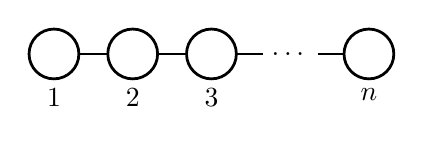
\begin{tikzpicture}
        %\GraphInit[vstyle=Classic]
        \SetVertexMath
        %\tikzset{VertexStyle/.style = {shape = circle,fill = black, minimum size = 5pt,inner sep=0pt}}
        %\SetVertexNoLabel
        \SetVertexLabelOut
        \SetVertexNormal[Shape=circle, FillColor=\off, LineWidth=1pt]
        \Vertex[Lpos=-90]{1}
        \EA[Lpos=-90](1) {2}
        \EA[Lpos=-90](2) {3}
        \SetGraphUnit{2}
        \EA[Lpos=-90](3) {n}
        \Edges(1,2,3)
        \Edge[label={\ldots}](3)(n)
    \end{tikzpicture}
    %\captionsetup{labelformat=empty}
\end{figure}
This is a tridiagonal matrix with $1$s on the diagonal, which we denote by $T_n$.
\end{frame}

\begin{frame}
\frametitle{When is the Linear Lightbulb Game Solvable?}
The determinant of $T_n$ is given by the recursive formula:
\[
    \abs{T_n} = \abs{T_{n-1}} - \abs{T_{n-2}}
\]
\pause
Seeing that $\abs{T_1} = 1$ and $\abs{T_2} = 0$, we get
\[
    \abs{T_n} = 
    \begin{cases}
        1 & n \equiv 0, 1 \pmod{6},\\
        0 & n \equiv 2, 5 \pmod{6},\\
        -1 & n \equiv 3,4 \pmod{6}.
    \end{cases}
\]
\pause
So the linear game is always solvable, unless $n \equiv 2 \pmod{3}$.
\end{frame}

\begin{frame}
    \frametitle{The Lightbulb Game on a Graph}

    We can further generalize this game by using a graph to specify which switches
    affect which lightbulbs:

    \begin{figure}[!h]
        \centering
        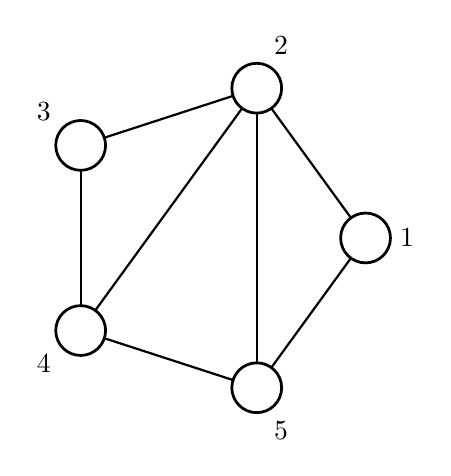
\begin{tikzpicture}
            %\GraphInit[vstyle=Classic]
            \SetVertexMath
            %\tikzset{VertexStyle/.style = {shape = circle,fill = black, minimum size = 5pt,inner sep=0pt}}
            %\SetVertexNoLabel
            \SetVertexLabelOut
            \SetGraphUnit{2}
            \begin{scope}[rotate=0]
                \SetVertexNormal[Shape=circle, FillColor=\off, LineWidth=1pt]
                \Vertices{circle}{1,2,3,4,5}
                \Edges(1,2,3,4,5,1) \Edges(5,2,4)
            \end{scope}
        \end{tikzpicture}
        %\captionsetup{labelformat=empty}
    \end{figure}
\end{frame}

\begin{frame}
    \frametitle{The Adjacency Matrix}
    The matrix $A$ in the linear system for this lightbulb game on a graph is
    represented by the adjacency matrix of the graph.
    \begin{figure}
        \begin{minipage}{.5\textwidth}
            \[
                \begin{pmatrix}
                    1 & 1 & 0 & 0 & 1\\
                    1 & 1 & 1 & 1 & 1\\
                    0 & 1 & 1 & 1 & 0\\
                    0 & 1 & 1 & 1 & 1\\
                    1 & 1 & 0 & 1 & 1
                \end{pmatrix}
            \]
        \end{minipage}%
        \begin{minipage}{.5\textwidth}
            \begin{figure}[!h]
                \centering
                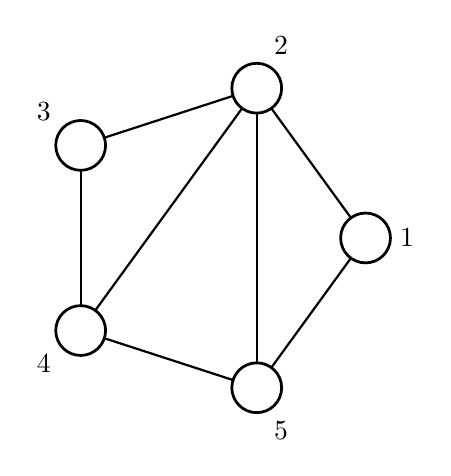
\begin{tikzpicture}
                    %\GraphInit[vstyle=Classic]
                    \SetVertexMath
                    %\tikzset{VertexStyle/.style = {shape = circle,fill = black, minimum size = 5pt,inner sep=0pt}}
                    %\SetVertexNoLabel
                    \SetVertexLabelOut
                    \SetGraphUnit{2}
                    \begin{scope}[rotate=0]
                        \SetVertexNormal[Shape=circle, FillColor=\off, LineWidth=1pt]
                        \Vertices{circle}{1,2,3,4,5}
                        \Edges(1,2,3,4,5,1) \Edges(5,2,4)
                    \end{scope}
                \end{tikzpicture}
                %\captionsetup{labelformat=empty}
            \end{figure}
        \end{minipage}
    \end{figure}
\end{frame}

\begin{frame}
    \frametitle{The Cyclic Lightbulb Game}
    We investigated the case where the graph is a cycle on $n$ vertices.

\begin{figure}[!h]
    \centering
    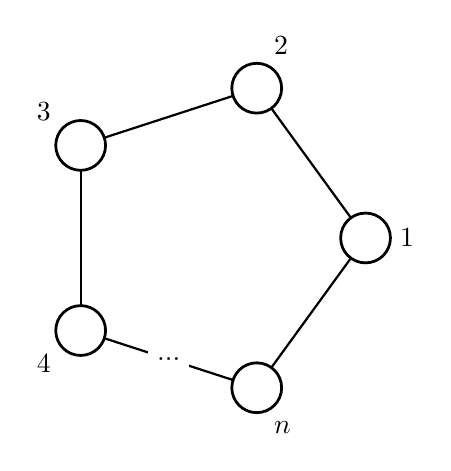
\begin{tikzpicture}
        %\GraphInit[vstyle=Classic]
        \SetVertexMath
        %\tikzset{VertexStyle/.style = {shape = circle,fill = black, minimum size = 5pt,inner sep=0pt}}
        %\SetVertexNoLabel
        \SetVertexLabelOut
        \SetGraphUnit{2}
        \begin{scope}[rotate=0]
            \SetVertexNormal[Shape=circle, FillColor=\off, LineWidth=1pt]
            \Vertices{circle}{1,2,3,4,n}
            \Edges(1,2,3,4) \Edges(n,1)
            \Edge[label={...}](4)(n)
        \end{scope}
    \end{tikzpicture}
    %\captionsetup{labelformat=empty}
\end{figure}
\end{frame}

%%%%%%%%%%%%%%%%%%%%%%%%%%%%%%%%%%%%

\begin{frame}
\frametitle{The Recursive Formula}

We will show the adjacency matrix $A_n$ of the cyclic graph $C_n$, has its determinant
given by
\[
    \abs{A_n} = \abs{T_{n-1}} - 2\abs{T_{n-2}} + 2(-1)^{n+1}
\]
\end{frame}

\begin{frame}
\frametitle{The Recursive Formula}
    $A_n$ has the form:
    \[
        A_n=
        \begin{pmatrix}
            1 & 1 & 0 & 0 & \dots & 0 & 1\\
            1 & 1 & 1 & 0 & \dots & \dots & 0\\
            0 & 1 & \ddots & \ddots & \ddots & \ddots & \vdots\\
            0 & 0 & \ddots & \ddots & \ddots & \vdots & \vdots\\
            \vdots & \vdots & \ddots & \ddots & \ddots & \ddots & 0\\
            0 & \vdots & \dots & \ddots & \ddots & \ddots & 1\\
            1 & 0 & \dots & \dots & 0 & 1 & 1
        \end{pmatrix}
    \]
\end{frame}

\begin{frame}
\frametitle{The Recursive Formula}
    We preform cofactor expansion along the first row of $A_n$. This will yield 3 terms.
    \[
        A_n=
        \left(\begin{array}{ccccccc}
            \rowcolor{red!20}
            1 & 1 & 0 & 0 & \dots & 0 & 1\\
            1 & 1 & 1 & 0 & \dots & \dots & 0\\
            0 & 1 & \ddots & \ddots & \ddots & \ddots & \vdots\\
            0 & 0 & \ddots & \ddots & \ddots & \vdots & \vdots\\
            \vdots & \vdots & \ddots & \ddots & \ddots & \ddots & 0\\
            0 & \vdots & \dots & \ddots & \ddots & \ddots & 1\\
            1 & 0 & \dots & \dots & 0 & 1 & 1
        \end{array}\right)
    \]
\end{frame}

\begin{frame}
\frametitle{The Recursive Formula}

    \bigskip

    \textbf{First term}
    \small
    \[
        A_n=
        \left(\begin{array}{>{\columncolor{red!20}}ccccccc}
            \rowcolor{red!20}
            1 & 1 & 0 & 0 & \dots & 0 & 1\\
            1 & 1 & 1 & 0 & \dots & \dots & 0\\
            0 & 1 & \ddots & \ddots & \ddots & \ddots & \vdots\\
            0 & 0 & \ddots & \ddots & \ddots & \vdots & \vdots\\
            \vdots & \vdots & \ddots & \ddots & \ddots & \ddots & 0\\
            0 & \vdots & \dots & \ddots & \ddots & \ddots & 1\\
            1 & 0 & \dots & \dots & 0 & 1 & 1
        \end{array}\right)
        \hspace{.1in}
        (-1)^{1+1}
        \begin{vmatrix}
            1 & 1 & 0 & \dots & 0\\
            1 & 1 & 1 & \ddots & \vdots\\
            0 & 1 & \ddots & \ddots  & 0\\
            \vdots & \ddots & \ddots & \ddots & 1\\
            0 & \dots & 0 & 1 & 1
        \end{vmatrix}
    \]
    \normalsize
    This is a tridiagonal matrix with ones on each diagonal. So this term is just
    $\abs{T_{n-1}}$.
\end{frame}


\begin{frame}
\frametitle{The Recursive Formula}
    \textbf{Second term}
    \small
    \[
        A_n=
        \left(\begin{array}{c>{\columncolor{red!20}}cccccc}
            \rowcolor{red!20}
            1 & 1 & 0 & 0 & \dots & 0 & 1\\
            1 & 1 & 1 & 0 & \dots & \dots & 0\\
            0 & 1 & \ddots & \ddots & \ddots & \ddots & \vdots\\
            0 & 0 & \ddots & \ddots & \ddots & \vdots & \vdots\\
            \vdots & \vdots & \ddots & \ddots & \ddots & \ddots & 0\\
            0 & \vdots & \dots & \ddots & \ddots & \ddots & 1\\
            1 & 0 & \dots & \dots & 0 & 1 & 1
        \end{array}\right)
        \hspace{.1in}
        (-1)^{1+2}
        \underbrace{
        \begin{vmatrix}
            1 & 1 & 0 & \dots & 0\\
            0 & 1 & 1 & \ddots & \vdots\\
            0 & 1 & \ddots & \ddots  & 0\\
            \vdots & \ddots & \ddots & \ddots & 1\\
            1 & \dots & 0 & 1 & 1
        \end{vmatrix}}_{\abs{B_{n-1}}}
    \]
    \normalsize
    We denote this matrix by $B_{n-1}$.
\end{frame}

\begin{frame}
\frametitle{The Recursive Formula}
    \textbf{Third term}
    \small
    \[
        A_n=
        \left(\begin{array}{cccccc>{\columncolor{red!20}}c}
            \rowcolor{red!20}
            1 & 1 & 0 & 0 & \dots & 0 & 1\\
            1 & 1 & 1 & 0 & \dots & \dots & 0\\
            0 & 1 & \ddots & \ddots & \ddots & \ddots & \vdots\\
            0 & 0 & \ddots & \ddots & \ddots & \vdots & \vdots\\
            \vdots & \vdots & \ddots & \ddots & \ddots & \ddots & 0\\
            0 & \vdots & \dots & \ddots & \ddots & \ddots & 1\\
            1 & 0 & \dots & \dots & 0 & 1 & 1
        \end{array}\right)
        \hspace{.1in}
        (-1)^{1+n}
        \underbrace{
        \begin{vmatrix}
            1 & 1 & 1 & \dots & 0\\
            0 & 1 & 1 & \ddots & \vdots\\
            0 & 0 & \ddots & \ddots  & 1\\
            \vdots & \ddots & \ddots & \ddots & 1\\
            1 & \dots & 0 & 0 & 1
        \end{vmatrix}}_{\abs{C_{n-1}}}
    \]
    \normalsize
    We denote this matrix by $C_{n-1}$.
\end{frame}

\begin{frame}
    \frametitle{The Recursive Formula}
    So far we have
    \[
        \abs{A_n} = \abs{T_{n-1}} - \abs{B_{n-1}} + (-1)^{n+1} \abs{C_{n-1}}
    \]
    We now perform cofactor expansion on $B_{n-1}$ and $C_{n-1}$ as well.
\end{frame}

\begin{frame}
\frametitle{The Recursive Formula}
    We expand on the first column of $B_{n-1}$, giving us two terms.
    \bigskip

    \textbf{First term}
    \small
    \[
        B_{n-1} = 
        \left(\begin{array}{>{\columncolor{red!20}}ccccccc}
            \rowcolor{red!20}
            1 & 1 & 0 & \dots & 0\\
            0 & 1 & 1 & \ddots & \vdots\\
            0 & 1 & \ddots & \ddots  & 0\\
            \vdots & \ddots & \ddots & \ddots & 1\\
            1 & \dots & 0 & 1 & 1
        \end{array}\right)
        \hspace{.1in}
        (-1)^{1+1}
        \begin{vmatrix}
            1 & 1 & 0 & \dots & 0\\
            1 & 1 & 1 & \ddots & \vdots\\
            0 & 1 & \ddots & \ddots & 0\\
            \vdots & \ddots & \ddots & \ddots & 1\\
            0 & \dots & 0 & 1 & 1
        \end{vmatrix}
    \]
    This is the tridiagonal matrix $T_{n-2}$.
    \normalsize
\end{frame}

\begin{frame}
\frametitle{The Recursive Formula}
    We expand on the first column of $B_{n-1}$, giving us two terms.
    \bigskip

    \textbf{Second term}
    \small
    \[
        B_{n-1} = 
        \left(\begin{array}{>{\columncolor{red!20}}ccccccc}
            1 & 1 & 0 & \dots & 0\\
            0 & 1 & 1 & \ddots & \vdots\\
            0 & 1 & \ddots & \ddots  & 0\\
            \vdots & \ddots & \ddots & \ddots & 1\\
            \rowcolor{red!20}
            1 & \dots & 0 & 1 & 1
        \end{array}\right)
        \hspace{.1in}
        (-1)^{n-1+1}
        \begin{vmatrix}
            1 & 0 & 0 & \dots & 0\\
            1 & 1 & 0 & \ddots & \vdots\\
            1 & \ddots & \ddots & \ddots & 0\\
            \vdots & \ddots & \ddots & \ddots & 0\\
            0 & \dots & 1 & 1 & 1
        \end{vmatrix}
    \]
    This is a lower triangular matrix with $1$s along the diagonal. So its determinant
    is $1$.
    \normalsize
\end{frame}

\begin{frame}
\frametitle{The Recursive Formula}

We have obtained the following formula for $\abs{B_{n-1}}$:
\[
    \abs{B_{n-1}} = \abs{T_{n-2}} + (-1)^n
\]
\end{frame}

\begin{frame}
\frametitle{The Recursive Formula}
    We expand on the first column of $C_{n-1}$, giving us two terms.
    \bigskip

    \textbf{First term}
    \small
    \[
        C_{n-1} = 
        \left(\begin{array}{>{\columncolor{red!20}}ccccccc}
            \rowcolor{red!20}
            1 & 1 & 1 & \dots & 0\\
            0 & 1 & 1 & \ddots & \vdots\\
            0 & 0 & \ddots & \ddots  & 1\\
            \vdots & \ddots & \ddots & \ddots & 1\\
            1 & \dots & 0 & 0 & 1
        \end{array}\right)
        \hspace{.1in}
        (-1)^{1+1}
        \begin{vmatrix}
            1 & 1 & 1 & \dots & 0\\
            0 & 1 & 1 & \ddots & \vdots\\
            0 & \ddots & \ddots & \ddots & 1\\
            \vdots & \ddots & \ddots & \ddots & 1\\
            0 & \dots & \dots & 0 & 1
        \end{vmatrix}
    \]
    This is an upper triangular matrix with $1$s along its diagonal. So its determinant
    is $1$.
    \normalsize
\end{frame}

\begin{frame}
\frametitle{The Recursive Formula}
    We expand on the first column of $C_{n-1}$, giving us two terms.
    \bigskip

    \textbf{Second term}
    \small
    \[
        C_{n-1} = 
        \left(\begin{array}{>{\columncolor{red!20}}ccccccc}
            1 & 1 & 1 & \dots & 0\\
            0 & 1 & 1 & \ddots & \vdots\\
            0 & 0 & \ddots & \ddots  & 1\\
            \vdots & \ddots & \ddots & \ddots & 1\\
            \rowcolor{red!20}
            1 & \dots & 0 & 0 & 1
        \end{array}\right)
        \hspace{.1in}
        (-1)^{n-1+1}
        \begin{vmatrix}
            1 & 1 & 0 & \dots & 0\\
            1 & 1 & 1 & \ddots & \vdots\\
            0 & 1 & \ddots & \ddots & 0\\
            \vdots & \ddots & \ddots & \ddots & 1\\
            0 & \dots & 0 & 1 & 1
        \end{vmatrix}
    \]
    This is the tridiagonal matrix $T_{n-2}$ again.
    \normalsize
\end{frame}

\begin{frame}
\frametitle{The Recursive Formula}

For $\abs{C_{n-1}}$ we have:
\[
    \abs{C_{n-1}} = 1 + (-1)^n\abs{T_{n-2}}
\]
\end{frame}

\begin{frame}
\frametitle{The Recursive Formula}

We substitute into the formula for $\abs{A_n}$:
\pause
    \begin{align*}
        \abs{A_n} &= \abs{T_{n-1}} - \abs{B_{n-1}} + (-1)^{n+1}\abs{C_{n-1}} \\
        &= \abs{T_{n-1}} - \left( \abs{T_{n-2}} + (-1)^n \right) + (-1)^{n+1}\left( 1 +
            (-1)^n \abs{T_{n-2}} \right)\\
        &= \abs{T_{n-1}} - \abs{T_{n-2}} + 2(-1)^{n+1} + (-1)^{2n+1}\abs{T_{n-2}}\\
        &= \abs{T_{n-1}} - 2\abs{T_{n-2}} + 2(-1)^{n+1}
    \end{align*}
    \pause
    But when is $\abs{A_n} = 0$? We claim if and only if $n \equiv 0 \pmod{3}$.
\end{frame}

\begin{frame}
\frametitle{The Recursive Formula}
Recall that $\abs{T_n}$ is given by 
\[
    \abs{T_n} = 
    \begin{cases}
        1 & n \equiv 0, 1 \pmod{6},\\
        0 & n \equiv 2, 5 \pmod{6},\\
        -1 & n \equiv 3,4 \pmod{6}.
    \end{cases}
\]
\end{frame}

\begin{frame}
\frametitle{The Recursive Formula}

$(\Rightarrow):$ If $\abs{A_n}=0$, then
\[
    \abs{A_n} = \abs{T_{n-1}} - 2\abs{T_{n-2}} + 2(-1)^{n+1} = 0
\]
\pause
But $\abs{T_{n-1}}$ and $\abs{T_{n-2}}$ only take on the values $0$,$1$, $-1$ so\ldots
\[
    \abs{A_n} = \{1,-1,0\} + \{2,-2,0\} + \{2,-2\} = 0
\]
\pause
So we must have that $\abs{T_{n-1}} = 0$. 
\pause

But then $n\equiv 0,3 \pmod{6}$ i.e. $n\equiv 0 \pmod{3}$.
\end{frame}

\begin{frame}
\frametitle{The Recursive Formula}

$(\Leftarrow):$ If $n\equiv 0 \pmod 3$ we have two possibilities for $n$ mod $6$:
\pause
\begin{enumerate}
    \item $n\equiv 0 \pmod{6}$, so $\abs{T_{n-1}} = 0$, $\abs{T_{n-2}}=-1$ and $n$ is
        even.
        \[ 
            \abs{A_n} = \abs{T_{n-1}} - 2\abs{T_{n-2}} + 2(-1)^{n+1} = 0 + 2 -2 = 0.
        \]
        \pause
    \item $n\equiv 3 \pmod{6}$, so $\abs{T_{n-1}} = 0$, $\abs{T_{n-2}}=1$ and $n$ is
        odd.
        \[ 
            \abs{A_n} = \abs{T_{n-1}} - 2\abs{T_{n-2}} + 2(-1)^{n+1} = 0 - 2 +2 = 0.
        \]
\end{enumerate}
\end{frame}


\end{document}


